\documentclass[11pt]{article}
\setlength\parindent{0pt}

\usepackage{amsmath}
\usepackage{amssymb}
\usepackage{algorithm}
\usepackage{algpseudocode}
\usepackage{tikz}
\usepackage{hyperref}

\graphicspath{{images/}}

\begin{document}
\title{Improving Web Scraping with Parallelism}
\author{Noah Christiano}
\date{April 18, 2018}
\maketitle

\section{Introduction}

Web scraping is a technique employed to extract data from websites for use off-line. The many components of web scrapers allows for lots of room for improvement. In order to discuss potential improvements, it is helpful first to define the architecture of a web scraper. \\

A web scraper consists of several somewhat independent components. This lends itself well to a modular design. The scraper typically takes input consisting of a set of URLs to be scraped and various parameters about how the scrape should be executed. The URLs are checked that they adhere to standards (that they are correct) and are then stored in a data structure, typically a queue. A requests module takes URLs from the data structure and attempts to download the HTML from the Internet. This HTML is then passed to a parsing pipeline that extracts the data of interest. The data is finally persisted locally, usually in a database. During parsing, links are typically scraped from the HTML and added to the URLs data structure, allowing the scraper to recursively crawl through the website. \\

This project focuses mainly on the request module and the data structure(s) for storing URLs. Most of the time during scraping is spent waiting on responses from websites. The problems posed by the other components of the scraper, such as parsing and parallel database storage, are widely studied. These components already have many thoughtful and performance-oriented solutions implemented in open source. \\

The goal of this project is to investigate how parallel programming models and data structures can be used to improve the performance of a web scraper. Performance is defined as the number of pages scraped per unit time. Several web scraping frameworks are already implemented in open source. However, these implementations primarily focus on usability and extensibility rather than performance. The two open source projects of interest are \href{https://scrapy.org/}{Scrapy} written in Python and \href{http://nutch.apache.org/}{Apache Nutch} written in Java.

\section{Architecture}

\begin{figure}[H]
	\centering
	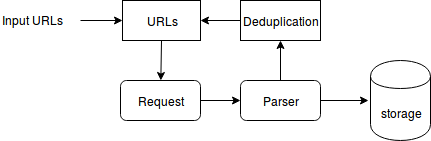
\includegraphics[scale=0.5]{simple_scraper}
	\caption{Architecture for a simple, serial web scraper}
\end{figure}

The simple architecture in Figure 1 adds one critical component to the web scraper that is not discussed in the introduction. There must be a data structure (`deduplication') that ensures that each URL is only scraped once by only allowing new URLs to be added to `URLs'. De-duplicating URLs is essential for ensuring that the webscraper does not loop infinitely. For example, on most websites there is a link to the homepage on every page.

\section{Algorithms and Data Structures}

The first step in building a web scraper would be parallelizing the request module. Web requests can be easily sent in parallel using a multi-processing or multi-threaded model. However, using one of these models requires that the set of URLs and the deduplication data structure allow for safe access in parallel. Additionally, the URLs set and deduplication data structure must be synchronized between threads to prevent duplicate URLs from being added to the URLs or URLs being scraped more than once by multiple requests modules. \\

The data structure best fitting for deduplication is a lock-free hash table. For storing URLs, a lock-free queue, such as the Michael \& Scott Lock-Free Queue, is best. Both the queue and hash table have $O(1)$ insertion and fetching, which is essential for the performance of the scraper. Due to the Internet's massive scale, even a logarithmic decrease in performance as the set of URLs grows would result in massive inefficiency. \\

In parallel, determining termination also becomes a problem. Checking if the URLs set is empty is insubstantial because another working thread could add more URLs to the URLs set. Misra Termination Detection is useful for accomplishing this goal.

\section{Implementation}

I implemented my parallel web scraper in C++. Most would advise against using C++ due to the amount of string manipulation involved in web scraping. It is much easier to build parsers in Python than C++. However, the focus of this project was on parallel systems and therefore it was only appropriate to use a systems programming language. \\

My implementation has six modules. \\

\textbf{\texttt{input.h}} \\
This module parses the input file.\\

\textbf{\texttt{scraper.cpp}} \\
This is the core of this project. It is responsible for launching the requesting threads using pthreads.\\

\textbf{\texttt{request.h}} \\
This module sends requests using curl and returns HTML to the scraping thread.\\

\textbf{\texttt{parser.h}} \\
This module parses HTML and extracts links using libxml2.\\

\textbf{\texttt{blocking\_queue.h}} \\
This queue contains the set of URLs to be scraped. \\

This module uses a shared mutex lock to make a thread safe queue. Although it would have been preferable to use an M\&S queue, I struggled to adapt my M\&S queue implementation to store strings.\\ 

\textbf{\texttt{shared\_map.h}} \\
This module contains a hashmap used to deduplicate URLs returned from the parser. \\

I used a shared mutex lock to make a thread safe hashmap. Like with the blocking queue, it would have been ideal for me to implement a lock-free hashmap.

\section{Results}

I tested my implementation on my personal machine and used an input list \texttt{urls.txt} of sites that are purpose built for testing web scrapers. Using test sites as opposed to real ones had several benefits. By using real websites, I was able to test how the parallel scraper handled the randomness bugginess of the Internet, which can be hard to simulate locally. Scraping websites not only is generally a massive waste of the hosts resources, but also can impact the browsing experience of human visitors. Picking websites purpose-built for testing scrapers helped handle this ethically ambiguous area around web scraping. \\

My machine has an Intel Core i7-4770K CPU with 8 threads. \texttt{Speedtest.net} reports my Internet speed as 900 Mbps down and 843 Mbps up, with an 8ms ping from Rochester, NY to Mansfield, PA. Average and standard deviation are calculated from five tests. 

\begin{center}
Parallel web scraper, \texttt{urls.txt} \\
\begin{tabular}{l|r|r}
Threads & Average & Standard Deviation \\
\hline
1 & 2336 & 7184.05 \\
2 & 10855 & 1232.12 \\
4 & 5420.2 & 807.79 \\
8 & 2617.2 & 36.72 \\
16 & 1428 & 74.1 \\
32 & 910.4 & 13.01 \\
64 & 5778.6 & 148.16 \\
\end{tabular}
\end{center}

I also ran \texttt{urls.txt} on Scrapy to compare the performance of my scraper with another open source package.

\begin{center}
Scrapy, \texttt{urls.txt} \\
\begin{tabular}{l|r|r}
Threads & Average & Standard Deviation \\
\hline
1 & 8247.2 & 831.06 \\
\end{tabular}
\end{center}

\begin{figure}[H]
	\centering
	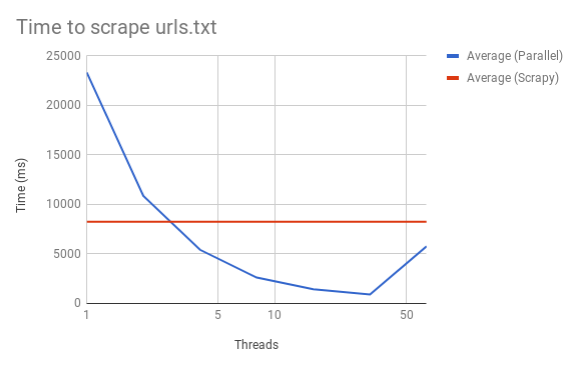
\includegraphics[scale=0.5]{graph_log}
\end{figure}

With a lower number of threads, the parallel scraper is likely slower that Scrapy due to the overhead caused by using a multi-threaded model and parallel data structures. It is interesting that the parallel scraper is faster with 32 threads than with 8 threads, despite that my CPU only has 8 threads. This could be the result of threads yielding the CPU to other threads while waiting on an HTTP responses.

\end{document}